\documentclass[a4paper,12pt]{article}
\usepackage[a4paper,top=1.3cm,bottom=2cm,left=1.5cm,right=1.5cm,marginparwidth=0.75cm]{geometry}
\usepackage{cmap}
\usepackage{mathtext}
\usepackage[T2A]{fontenc}
\usepackage[utf8]{inputenc}
\usepackage[english,russian]{babel}
\usepackage{siunitx}

\usepackage{graphicx}

\usepackage{wrapfig}
\usepackage{tabularx}
\usepackage{multirow}

\usepackage{hyperref}
\usepackage[rgb]{xcolor}
\hypersetup{
colorlinks=true,urlcolor=blue
}
\usepackage{amsmath,amsfonts,amssymb,amsthm,mathtools}
\usepackage{icomma}
\mathtoolsset{showonlyrefs=false}
\usepackage{euscript}
\usepackage{mathrsfs}
\DeclareMathOperator{\sgn}{\mathop{sgn}}
\newcommand*{\hm}[1]{#1\nobreak\discretionary{}
{\hbox{$\mathsurround=0pt #1$}}{}}

%%% Заголовок
\author{Макаров Лев Евгеньевич}
\title{Лабораторная работа №1.2.5

Изучение экспериментальных погрешностей на примере физического маятника
}
\date{\today}

\begin{document}

\begin{titlepage}
	\begin{center}
		{\large МОСКОВСКИЙ ФИЗИКО-ТЕХНИЧЕСКИЙ ИНСТИТУТ (НАЦИОНАЛЬНЫЙ ИССЛЕДОВАТЕЛЬСКИЙ УНИВЕРСИТЕТ)}
	\end{center}
	\begin{center}
		{\large Физтех-школа фотоники, электроники и молекулярной физики}
	\end{center}
	
	
	\vspace{4.5cm}
	{\huge
		\begin{center}
			{\bf Отчёт о выполнении лабораторной работы 1.4.8}\\
			Измерение модуля Юнга методом аккустического резонанса
		\end{center}
	}
	\vspace{2cm}
	\begin{flushright}
		{\LARGE Автор:\\ Макаров Лев Евгеньевич \\
			\vspace{0.2cm}
			Б04-306}
	\end{flushright}
	\vspace{8cm}
	\begin{center}
		Долгопрудный 2023
	\end{center}
\end{titlepage}

\section{Введение}

\textbf{Цель работы:} 
\begin{enumerate}
	\item исследовать явление акустического резонанса в тонком стержне
	\item измерить скорость распространения продольных звуковых колебаний в тонких стержнях из различных материалов и различных размеров
    \item измерить модули Юнга различных материалов
\end{enumerate}

\textbf{В работе используются:} 
\begin{itemize}
    \item генератор звуковых частот
    \item частотомер
    \item осциллограф
    \item электромагнитные излучатель и приёмник колебаний
    \item набор стержней из различных материалов
\end{itemize}
\medskip

\section{Теоретические сведения}

Согласно закону Гука при приложении к элементу среды механического напряжения $\sigma$ возникает относительная деформация в этом направлении $\varepsilon = \frac{\Delta x}{x_0}$, определяемая соотношением

\begin{equation}\label{law}
    \sigma = \varepsilon E
\end{equation}

При кратковременном воздействии в среде возникает кратковременная волна, называемая аккустической или звуковой. Скорость распространения этой волны $u$ равна

\begin{equation}\label{e-u-rho}
    u = \sqrt{\frac{E}{\rho}}
\end{equation}

где $\rho$ -- плотность среды.

Рассмотрим стержень длинной $L$. Его можно считать тонким в направлении распространения волн, если длина $\lambda$ звуковых волн в нём сильно больше радиуса: $\lambda \gg R$. Такая волна может распространяться только вдоль стержня.

Аккустическая волна отражается от торцов стержня. Если при этом на длине стержня укладывается целое число полуволн, то отражённые волны будут складываться в фазе с падающими, что приведёт к резкому усилению амплитуды их колебаний и возникновению акустического резонанса в стержне. Измеряя соответствующие резонансные частоты, можно определить скорость звуковой волны в стержне и, таким образом, измерить модуль Юнга материала стержня. Акустический метод является одним из наиболее точных методов определения упругих характеристик твёрдых тел.

Волновое уравнение выглядит так:

\begin{equation}\label{wave-eq}
    \frac{\partial^2 \xi}{\partial t^2} = u^2 \frac{\partial^2 \xi}{\partial x^2}
\end{equation}

Здесь $\xi(x, t) = f(x - ut)$, где $f$ -- произвольная функция. Это дифференциальное уравнение описывает распространение упругих волн в тонком стержне. Оно имеет универсальный характер и описывает волны самой разной природы: акустические волны в твёрдых телах, жидкостях и газа, волны на струне, электромагнитные волны и т.п. Величина $u$ в уравнении \eqref{wave-eq} имеет смысл скорости распространения волны.


В случае гармонического возбуждения колебаний с частотой $f$ продоль-
ная волна в тонком стержне может быть представлена в виде суперпозиции
двух бегущих навстречу гармонических волн:

\begin{equation}\label{harmonic-waves}
    \xi(x, t) = A_1 \sin{\omega t - kx + \varphi_1} + A_2 \sin{\omega t - kx + \varphi_2}
\end{equation}

где $\omega = 2 \pi f$ -- циклическая частота. $k = 2 \pi / \lambda$ -- волновое число.


Первое слагаемое \eqref{harmonic-waves} описывает гармоническую (синусоидальную) волну, бегущую в положительном направлении по $x$, второе — в отрицательном. Соотношения между амплитудами $A_\text{1,2}$ и начальными фазами $\varphi_\text{1,2}$ этих волн, а также возможные частоты колебаний $\omega$, определяются граничными условиями на концах стержня. Рассмотрим этот вопрос подробнее.


Пусть концы стержня не закреплены. Тогда напряжения в них должны равняться нулю. Положим координаты торцов равными $x = 0$ и $x = L$. Тогда, используя связь напряжения и деформации 

\begin{equation}
    \sigma = \varepsilon E = E \frac{\partial \xi}{\partial x}
\end{equation}

запишем граничные условия для свободных (незакреплённых) концов стержня:

\begin{equation}\label{limits}
    \sigma(0) = 0 \longrightarrow \frac{\partial \xi}{\partial x} \left |_{_{x = 0}} = 0, \ \ \ \sigma(L) = 0 \longrightarrow \frac{\partial \xi}{\partial x} \right |_{x = L}
\end{equation}

Соотношения \eqref{limits} должны выполняться в произвольный момент времени. Записывая первое граничное условие \eqref{limits} для функции \eqref{harmonic-waves}, найдём

\begin{equation}
    -k A_1 \cos{\omega t + \varphi_1} + k A_2 \cos{\omega t + \varphi_2} = 0
\end{equation}

Нетрудно видеть, что это соотношение будет выполняться при любом $t$, если только у «падающей» и «отражённой» волн одинаковы амплитуды

\begin{equation}\label{same-amp}
    A_1 = A_2
\end{equation}

и фазы

\begin{equation}\label{same-phi}
    \varphi_1 = \varphi_2
\end{equation}

Условие равенства амплитуд \eqref{same-amp} можно интерпретировать как условие отражения волн от торцов без потери энергии. Поскольку на практике потери неизбежны, это условие выполняется лишь приближённо: $A_1 \approx A_2$. Условие \eqref{same-phi} означает, что при отражении синусоидальной волны от свободного конца стержня, её фаза не изменяется. Нетрудно также убедиться, что если же концы стержня закрепить $\left ( \xi \big|_{x = 0} = \xi \big|_{x = L} = 0 \right )$, то фазы падающей и отражённой волн будут отличаться друг от друга на $\pi$.

Далее, перепишем исследуемую функцию \eqref{harmonic-waves}, используя граничные условия \eqref{same-amp} и \eqref{same-phi} и формулу суммы синусов:

\begin{equation}\label{harmonic-waves-2}
    \xi (x, t) = 2 A \cos{kx} \sin{\omega t + \varphi}
\end{equation}

Колебания вида \eqref{harmonic-waves-2} называют гармоническими стоячими волнами. Наконец, воспользуемся вторым граничным условием \eqref{limits} применительно к функции \eqref{harmonic-waves-2}. В результате придём к уравнению $\sin{kL} = 0$, решения которого определяют набор допустимых значений волновых чисел $k$:

\begin{equation}\label{k}
    k_n L = \pi n, \ \ \ n \in \mathbb{N}
\end{equation}

или, выражая (13) через длину волны $\lambda = 2 \pi / k$, получим

\begin{equation}
    \lambda_n = \frac{2L}{n}, \ \ \ n \in \mathbb{N}
\end{equation}

Таким образом, для возбуждения стоячей волны на длине стержня должно укладываться целое число полуволн. 

Допустимые значения частот

\begin{equation}\label{linear-f}
    f_n = \frac{u}{\lambda_n} = n \frac{u}{2L}, \ \ \ n \in \mathbb{N}
\end{equation}

называют собственными частотами колебаний стержня длиной $L$. Именно при совпадении внешней частоты с одной из частот $f_n$ в стержне возникает акустический резонанс.

\begin{figure}[h!]
        \centering
	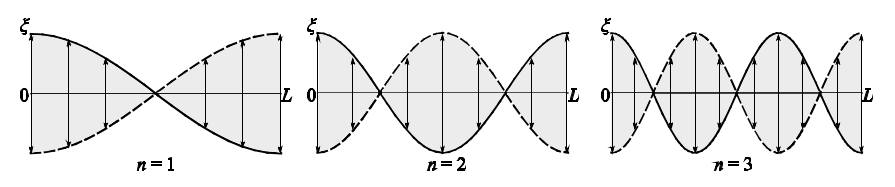
\includegraphics[width=0.6\textwidth]{waves.png}
	\caption{\textit{Собственные продольные колебания стержня с незакреплёнными концами (для наглядности изображение дано не в масштабе, реальные смещения малы по сравнению с длиной стержня, $\xi \ll L$)}}
	\label{waves}
\end{figure}

Зависимость амплитуды смещения $\xi$ от координаты $x$ для собственных колебаний стержня с незакреплёнными концами при $n = 1,2,3$ представлена на рис. \ref{waves}. Амплитуда колебаний смещения среды распределена вдоль стержня по гармоническому закону: $\xi_0 (x) = 2A \cos{kx}$. Точки с максимальной амплитудой называются пучностями смещения, точки с минимальной (нулевой) амплитудой — узлами смещения. Номер гармоники $n$ определяет количество узлов смещения на стержне. Заметим, что согласно закону Гука \eqref{law} в пучности смещения имеет место узел напряжения, и, наоборот, в узлах смещения имеется пучность напряжения (в частности, на свободных торцах стержня напряжение всегда нулевое, а деформация максимальна).

Напоследок отметим, что в реальной системе стоячая волна не может быть получена в чистом виде: всегда существуют потери энергии, связанные, в том числе с отражением волн на краях стержня $(A_1 \neq A_2)$. Поэтому для поддержания колебаний необходимо наличие некоторого стороннего возбудителя, а к стоячей волне примешивается бегущая с малой амплитудой: $\left | A_1 - A_2 \right | \ll A_{1,2}$. Также именно благодаря бегущим волнам энергия может передаваться от одних частей стержня к другим (в стоячей волне энергия не переносится, а только переходит из кинетической в потенциальную и обратно).

\section{Оборудование и экспериментальные погрешности}

\textbf{Штангенциркуль:} $\sigma_\text{шт} = \pm 0,005$ см \\
\textbf{Электронные весы ВЛТЭ-310:} $\sigma_m = \pm 0,003$ г \\
\textbf{Микрометр:} $\Delta_\text{мкм} = \pm 0,01 $ мм \\
\textbf{Измеритель частоты:} $\Delta_\text{ч} = \pm 0,3 $ Гц \\

\section{Результаты измерений и обработка данных}

\subsection{Настройка осциллографа}

Проведём предварительную настройку осциллографа. Выставим настройки согласно рисунку \ref{oscillator}. Таким образом при включении установки в дальнейшем мы получим фигуру Лиссажу на экране. Включим все приборы.

\begin{figure}[h!]
        \centering
	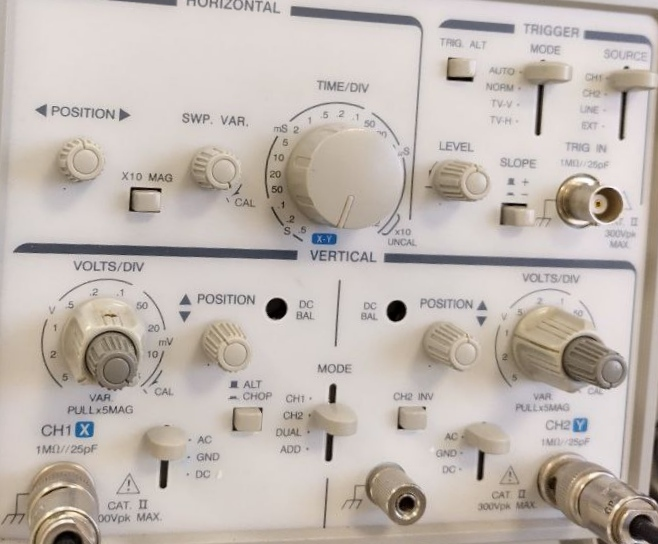
\includegraphics[width=0.6\textwidth]{oscillator-settings.jpg}
	\caption{\textit{Предварительные настройки осциллографа}}
	\label{oscillator}
\end{figure}

\subsection{Подготовка эксперимента}
\label{expirement-two}

Развдинем датчики и поместим между ними на подставку исследуемый стержень. В начале используется медный стержень. Длина стержня $L = (600 \pm 0,5) \text{ мм}$.

\subsection{Установка электромагнитов}

Разместим электромагниты напротив торцов стержня так, чтобы торцы стержня совпали с центрами датчиков, а зазор между полюсами электромагнита и торцевой поверхностью стержней составлял 1–3 мм. Плоскость магнитов должна быть строго перпендикулярна оси стержня. Электромагниты не должны касаться стержня.

\subsection{Предварительная оценка резонансных частот}

Для этого оценим частоту первого резонанса $f_1 = u / 2L$, где $u$ -- табличное значение скорости звука в среде. Для меди $u = 3790$ м/с. А значит $f_1 \approx 3160$ Гц. Значит резонансную частоту для стержня будем искать в этом диапазоне значений.

\subsection{Настройка утановки}

Медленно перестраивая звуковой генератор вблизи оценочного значения $f_1$ найдём первый резонанс. Приближение к резонансу характеризуется появлением фигуры Лиссажу на экране осциллографа. Для увеличения сигнала колебаний стержня нужно очень осторожно придвигать датчики к торцам стержня, не допуская прилипания стержня к датчикам. На экране осциллографа должна получиться фигура, напоминающая бочку (рис. \ref{barrel}). При резонансе амплитуда принятого сигнала достигает максимума и не меняется во времени.

\begin{figure}[h!]
        \centering
	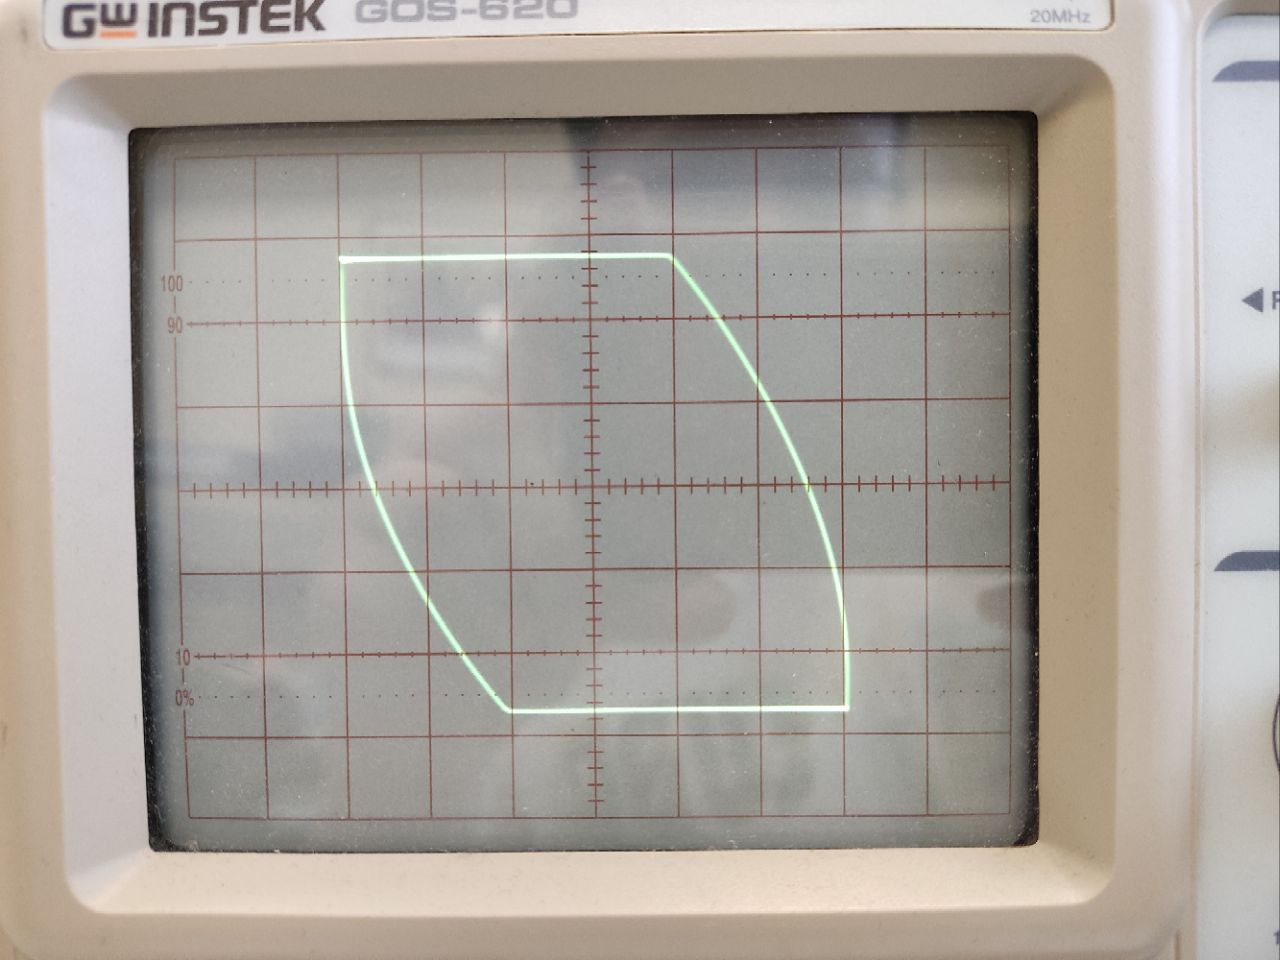
\includegraphics[width=0.6\textwidth]{barrel.jpg}
	\caption{\textit{Бочка}}
	\label{barrel}
\end{figure}

\subsection{Получение первого резонанса}

Согласно предыдущему пункту определим значение первого резонанса. 

\begin{equation}
    f_1 = 3218,7 \text{ Гц}
\end{equation}

Погрешность измерения равна утроенному последнему разряду измерения: $\sigma_{f_1} = 0,3 \text{ Гц}$.

\subsection{Определение резонансных частот}

Для определения значения резонансных частот оценим следующие значения по формуле:

\begin{equation}
    f_n = n f_1
\end{equation}

После чего будем искать резонанс в районе полученных значений по аналогии с первым резонансом и результаты измерений запишем в таблицу \ref{cu-resonance}.

\begin{table}[!ht]
    \centering
    \begin{tabular}{|l|l|l|l|l|l|l|l|}
    \hline
        n & 1 & 2 & 3 & 4 & 5 & 6 & 7 \\ \hline
        f, Гц & 3218,7 & 6444,2 & 9663,7 & 12890,0 & 16105,0 & 19308,0 & 22472,0 \\ \hline
    \end{tabular}\caption{\textit{Результаты измерения резонансных частот для медного стержня}}\label{cu-resonance}
\end{table}

Погрешность измерений равна $\sigma_f = 0,3$ Гц.

\subsection{Определение плотности стержня}

Плотность стержня будем определять используя несколько циллиндрических образцов, сделанных из того же материала, что и стержень. Для каждого измерим: диаметр с помощью микрометра, высоту с помощью штангенциркуля и массу с помощью электронных весов. После чего посчитаем плотность по формуле:

\begin{equation}
    \rho = \frac{4 m}{\pi h d^2}
\end{equation}

Приборную погрешность измерения плотности вычислим по формуле:

\begin{equation}
    \sigma_\rho^\text{приб} = \sqrt{
    \left ( \frac{\partial \rho}{\partial m} \right )^2 \sigma_{m} ^ 2 + 
    \left ( \frac{\partial \rho}{\partial h} \right )^2 \sigma_{h} ^ 2 + 
    \left ( \frac{\partial \rho}{\partial d} \right )^2 \sigma_{d} ^ 2
    }
\end{equation}

Результаты всех измерений запишем в таблицу \ref{density}.

\begin{table}[!ht]
    \centering
    \begin{tabular}{|l|l|l|l|l|l|l|l|l|}
    \hline
        n & 1 & 2 & 3 & 4 & 5 & 6 & 7 & 8 \\ \hline
        d, мм & 11,85 & 11,96 & 11,85 & 11,75 & 12,11 & 11,96 & 11,94 & 11,95 \\ \hline
        h, мм & 29,8 & 30,3 & 30,1 & 40,3 & 40,0 & 40,5 & 39,7 & 41,5 \\ \hline
        m, г & 29,109 & 30,106 & 29,453 & 38,710 & 40,989 & 40,347 & 39,382 & 41,333 \\ \hline
        $\rho$, $\text{кг}/\text{м}^3$ & 8857 & 8844 & 8872 & 8858 & 8897 & 8868 & 8859 & 8880 \\ \hline
        $\sigma_\rho^\text{приб}$, $\text{кг}/\text{м}^3$ & 33 & 33 & 33 & 27 & 27 & 26 & 27 & 26 \\ \hline
    \end{tabular}\caption{\textit{Измерение плотности стержня}}\label{density}
\end{table}

Среднее значение $\overline{\rho} = 8867$ $\text{кг}/\text{м}^3$. Тогда случайную погрешность можно вычислить по формуле: $ \sigma_\rho^\text{сл} = \sqrt{\frac{1}{N  (N-1)}\sum(\rho_i-\overline{\rho})^2} \approx 6 \text{ кг}/\text{м}^3$.

Тогда погрешность измерения плотности $\sigma_\rho = \sqrt{(\sigma_\rho^\text{сл})^2 + (\overline{\sigma_\rho^\text{приб}})^2} \approx 30 \text{ кг}/\text{м}^3 $. Тогда плотность медного стержня равна:

\begin{equation}
    \rho_\text{м} = (8867 \pm 30) \ \frac{\text{кг}}{\text{м}^3}
\end{equation}

\subsection{Проверка справедливости соотношения $R/\lambda \ll 1$}
\label{expirement-ten}

Диаметр стержня напрямую не измерялся но он сравним с диаметром образцов $d \approx 12 \text{мм}$. Длина волны при резонансе $\lambda$ вычисляется по формуле:

\begin{equation}
    \lambda = \frac{2 L}{n} \ \ \implies \ \ \frac{R}{\lambda} = \frac{R n}{2 L} = \frac{d n}{4 L} 
\end{equation}

Тогда если это соотношение выполняется для наибольшего $n$, то и для всех меньших значений оно тоже выполняется:

\begin{equation}
    \lambda = \frac{d n}{4 L} \approx 0,035 \ll 1
\end{equation}

Отсюда следует, что соотношение выполняется для всех $n <= 7$. Поэтому во время работы стержень можем считать тонким.

\subsection{Опыты с другими стержнями}

Повторим опыты пунктов \ref{expirement-two}-\ref{expirement-ten} для двух других стержней: стального и дюралюминиего.

Для обоих стержней измерим значение семи резонансных частот аналогично медному и запишем в таблицу \ref{al-fe-resonance}.

\begin{table}[!ht]
    \centering
    \begin{tabular}{|l|l|l|l|l|l|l|l|}
    \hline
        n & 1 & 2 & 3 & 4 & 5 & 6 & 7 \\ \hline
        $f_\text{ст}$, Гц & 4128,6 & 8285,1 & 12400,0 & 16529,0 & 20653,0 & 24772,0 & 28882,0 \\ \hline
        $f_\text{дюр}$, Гц & 4246,2 & 8514,2 & 12742,0 & 16998,0 & 21225,0 & 25453,0 & 29662,0 \\ \hline
    \end{tabular}\caption{\textit{Результаты измерения резонансных частот для двух стержней}}\label{al-fe-resonance}
\end{table}

Измерим плотность стержней аналогично медному, результаты измерений для стального запишем в таблицу \ref{steel-density}, а для дюралюминиего в таблицу \ref{dural-density}.

\begin{table}[!ht]
    \centering
    \begin{tabular}{|l|l|l|l|l|l|l|l|l|}
    \hline
        n & 1 & 2 & 3 & 4 & 5 & 6 & 7 & 8 \\ \hline
        d, мм & 11,98 & 11,83 & 11,99 & 12,00 & 12,00 & 11,99 & 11,89 & 12,11 \\ \hline
        h, мм & 29,6 & 32,2 & 29,9 & 40,0 & 39,7 & 39,9 & 41,1 & 41,3 \\ \hline
        m, г & 26,022 & 28,105 & 26,151 & 35,186 & 34,938 & 35,145 & 36,916 & 37,080 \\ \hline
        $\rho$, $\text{кг}/\text{м}^3$ & 7799 & 7941 & 7746 & 7778 & 7781 & 7801 & 8089 & 7795 \\ \hline
        $\sigma_\rho^\text{приб}$, $\text{кг}/\text{м}^3$ & 29 & 28 & 29 & 23 & 24 & 23 & 24 & 23 \\ \hline
    \end{tabular}\caption{\textit{Результаты измерения плотности стального стержня}}\label{steel-density}
\end{table}

Среднее значение $\overline{\rho}_\text{ст} = 7841$ $\text{кг}/\text{м}^3$. Тогда случайную погрешность можно вычислить по формуле: $ \sigma_\rho^\text{сл} = \sqrt{\frac{1}{N  (N-1)}\sum(\rho_i-\overline{\rho})^2} \approx 41 \text{ кг}/\text{м}^3$.

Тогда погрешность измерения плотности $\sigma_\rho = \sqrt{(\sigma_\rho^\text{сл})^2 + (\overline{\sigma_\rho^\text{приб}})^2} \approx 48 \text{ кг}/\text{м}^3 $. Тогда плотность стального стержня равна:

\begin{equation}
    \rho_\text{ст} = (7841 \pm 48) \ \frac{\text{кг}}{\text{м}^3}
\end{equation}

\begin{table}[!ht]
    \centering
    \begin{tabular}{|l|l|l|l|l|l|l|l|l|}
    \hline
        n & 1 & 2 & 3 & 4 & 5 & 6 & 7 & 8 \\ \hline
        d, мм & 12,05 & 11,85 & 11,73 & 11,73 & 11,85 & 11,74 & 11,75 & 12,12 \\ \hline
        h, мм & 30,1 & 30,1 & 30,1 & 30,8 & 40,1 & 41,4 & 41,5 & 41,2 \\ \hline
        m, г & 9,485 & 9,193 & 8,992 & 9,260 & 12,178 & 12,452 & 12,480 & 13,232 \\ \hline
        $\rho$, $\text{кг}/\text{м}^3$ & 2763 & 2769 & 2764 & 2782 & 2754 & 2779 & 2773 & 2784 \\ \hline
        $\sigma_\rho^\text{приб}$, $\text{кг}/\text{м}^3$ & 10 & 10 & 10 & 10 & 8 & 8 & 8 & 8 \\ \hline
    \end{tabular}\caption{\textit{Результаты измерения плотности дюралюминиего стержня}}\label{dural-density}
\end{table}

Среднее значение $\overline{\rho}_\text{дюр} = 2771$ $\text{кг}/\text{м}^3$. Тогда случайную погрешность можно вычислить по формуле: $ \sigma_\rho^\text{сл} = \sqrt{\frac{1}{N  (N-1)}\sum(\rho_i-\overline{\rho})^2} \approx 4 \text{ кг}/\text{м}^3$.

Тогда погрешность измерения плотности $\sigma_\rho = \sqrt{(\sigma_\rho^\text{сл})^2 + \langle\sigma_\rho^\text{приб})^2} \approx 10 \text{ кг}/\text{м}^3 $. Тогда плотность дюралюминиего стержня равна:

\begin{equation}
    \rho_\text{дюр} = (2771 \pm 10) \ \frac{\text{кг}}{\text{м}^3}
\end{equation}

Так как диаметр стержней одинаковый, а длина волн при резонансе такая же, то соотношение $R/\lambda \ll 1$ выполняется для обоих стержней. 

\subsection{Половинная частота резонанса}

Для стержня из дюралюминия проведём дополнительный опыт: добъёмся резонанса при частоте генератора $f = f_1 / 2 = 2123,5$ Гц. При этой частоте наблюдается фигура Лиссажу изображённая на рисунке \ref{butterfly}.

\begin{figure}[h!]
        \centering
	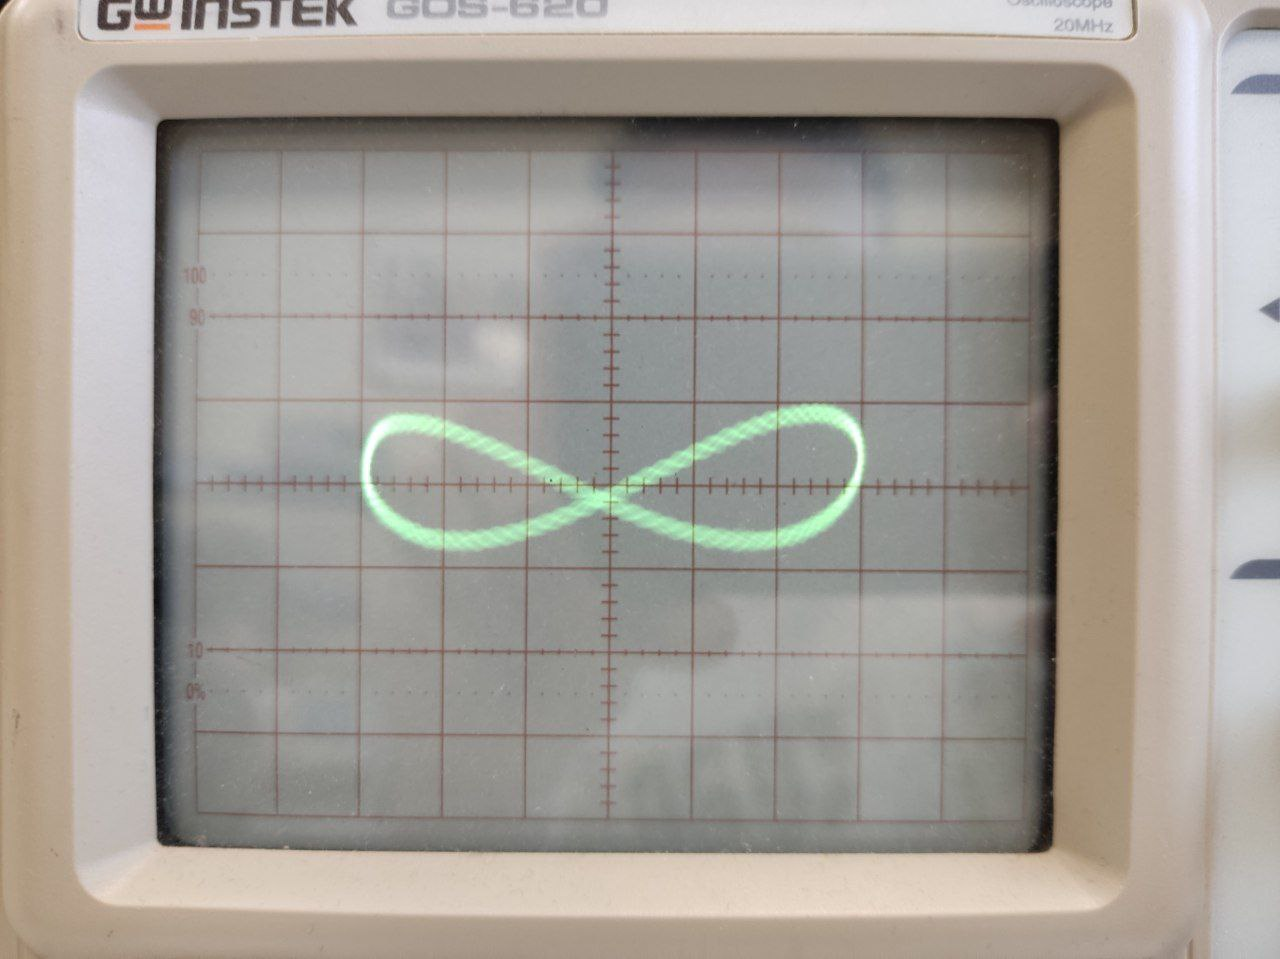
\includegraphics[width=0.6\textwidth]{butterfly.jpg}
	\caption{\textit{Фигура Лиссажу при половинном резонансе}}
	\label{butterfly}
\end{figure}

Во время обычного резонанса частота собственных колебаний стержня равна частоте колебаний стоячих волн в нём. Во время же половинного резонанса, частота колебаний волн в два раза больше. Из-за этого вид фигуры Лиссажу меняется: она становится похожа на бабочку (рис. \ref{butterfly}).

\subsection{Определение добротности стержня}

Для стального стержня определим добротность, как для колебательной системы, измерив амплитудно-частотную характеристику $A(f - f_1)$ вблизи первого резонанса. 

Ширина максимума функции $A(f - f_1)$ связана с добротностью $Q$ стержня как колебательной системы :

\begin{equation}\label{q}
    Q = \frac{f_n}{\Delta f}
\end{equation}

где $\Delta f$ -- ширина АЧХ на уровне $A = A_{max}/\sqrt{2}$. 

Получим резонанс в стержне при некоторой частоте $f = (4129 \pm 0,3)$ Гц и, переключив CH1 в режим GND считаем показания $A_{max} = (27 \pm 1)$ делений, соответственно $A \approx 19$ делений. Измерим $\Delta f = f_1 - f_2$. Где $f_1$ и $f_2$ - частоты, при которых достигается значение $A$. Погрешность измерения $\Delta f$ равна удвоенной погрешности измерения $f$: $\sigma_{\Delta f} = 0,6$ Гц. Повторим это измерение три раза и результаты запишем в таблицу \ref{width-A}.

\begin{table}[!ht]
    \centering
    \begin{tabular}{|l|l|l|l|}
    \hline
        № & 1 & 2 & 3 \\ \hline
        $f_1$, Гц & 4127,3 & 4127,4 & 4127,3 \\ \hline
        $f_2$, Гц  & 4130,3 & 4130,5 & 4130,4 \\ \hline
        $\Delta f$, Гц & 3,0 & 3,1 & 3,1 \\ \hline
        $Q$ & 1376 & 1332 & 1332 \\ \hline
        $\sigma_Q^\text{приб}$ & 138 & 129 & 129 \\ \hline
    \end{tabular}\caption{\textit{Измерение ширины АЧХ при $A$}}\label{width-A}
\end{table}


Для каждого измерения так же вычислим добротность по формуле \eqref{q}, где $f_n = f$ и результаты запишем в таблицу.

Приборную погрешность измерения $Q$ можно вычислить по формуле:

\begin{equation}
    \sigma_Q^\text{приб} = Q \sqrt{\left ( \frac{\sigma_f}{f} \right )^2 + \left ( \frac{\sigma_{\Delta f}}{\Delta f} \right )^2 }
\end{equation}

Вычислим её для каждого $Q$ и результаты запишем в таблицу. Случайная погрешность $Q$ пренебрежимо мала по сравнению с приборной, поэтому $\sigma_Q \approx \sigma_Q^\text{приб}$. Тогда добротность равна:

\begin{equation}
    Q = 1347 \pm 132
\end{equation}

\subsection{Опыты со стержнями другой длины}

Во врмея выполнения работы аналогичные опыты со стержнями с другими параметрами не проводились.

\subsection{Обработка результатов}

Для каждого из исследуемых стержней построим график зависимости $f_n$ от $n$. Для этого воспользуемся МНК. В данном случае $u = f_n$, а $v = n$. Так как зависимость согласно формуле должна быть линейной, получаем:

\begin{equation}
    k_\text{мед} = \frac{\langle uv\rangle}{\langle v^2 \rangle} = 3217 \ \text{Гц}
\end{equation}

\begin{equation}
    k_\text{ст} = \frac{\langle uv\rangle}{\langle v^2 \rangle} = 4129 \ \text{Гц}
\end{equation}

\begin{equation}
    k_\text{дюр} = \frac{\langle uv\rangle}{\langle v^2 \rangle} = 4243 \ \text{Гц}
\end{equation}

Найдём погрешность $\sigma_k$:

\begin{equation}
    \sigma_{k_\text{мед}} = \frac{1}{\sqrt{7}} \sqrt{\frac{\langle u^2 \rangle}{\langle v^2 \rangle} - k^2} = 2 \ \text{Гц}
\end{equation}

\begin{equation}
    \sigma_{k_\text{ст}} = \frac{1}{\sqrt{7}} \sqrt{\frac{\langle u^2 \rangle}{\langle v^2 \rangle} - k^2} = 1 \ \text{Гц}
\end{equation}

\begin{equation}
    \sigma_{k_\text{дюр}} = \frac{1}{\sqrt{7}} \sqrt{\frac{\langle u^2 \rangle}{\langle v^2 \rangle} - k^2} = 2 \ \text{Гц}
\end{equation}

График изображён на рисунке \ref{graph}.

\subsection{Определение скорости звука}

Определим скорость звука в стержнях. Для этого воспользуемся формулой \eqref{linear-f}. Оттуда следует, что:

\begin{equation}
    k = \frac{u}{2 L} \ \ \ \implies \ \ \ u = 2 L k
\end{equation}

Тогда случайная относительная погрешность $\varepsilon_u = \varepsilon_k^\text{случ}$. 

Коэффициент $k$ так же можно найти как $k = f_n / n$, поэтому приборная относительная погрешность $k$ равна приборной относительной погрешности $f_n$: $\varepsilon_k^\text{приб} = 0,01 \%$. Тогда

\begin{equation}
    \varepsilon_k = \sqrt{\left ( \varepsilon_k^\text{случ}\right )^2 + \left ( \varepsilon_k^\text{приб}\right )^2}
\end{equation}

Погрешность вычисления $u$ равна:

\begin{equation}
    \sigma_u = u \sqrt{\left ( \varepsilon_L \right )^2 + \left ( \varepsilon_k \right )^2}
\end{equation}

Для каждого стержня рассчитаем $u$ и $\sigma_u$, результаты измерений запишем в таблицу \ref{speed-sound}.

\begin{table}[!ht]
    \centering
    \begin{tabular}{|l|l|l|l|}
    \hline
        материал & медь & сталь & дюраль \\ \hline
        $k$, Гц & 3217 & 4129 & 4243 \\ \hline
        $\varepsilon_k$, $\%$ & 1 & 1 & 1 \\ \hline
        $u$, $\text{м}/\text{с}$ & 3860 & 4955 & 5092 \\ \hline
        $\sigma_u$, $\text{м}/\text{с}$ & 39 & 50 & 51 \\ \hline
    \end{tabular}\caption{\textit{Скорость звука в стержнях}}\label{speed-sound}
\end{table}

\subsection{Определение модуля Юнга}

Модуль Юнга для каждого стержня можно вычислить из формулы \eqref{e-u-rho}: $E = u^2 \rho$

Погрешность нахождения модуля Юнга можно найти по формуле:

\begin{equation}
    \sigma_E = \sqrt{
    \left ( \frac{\partial E}{\partial u} \right )^2 \sigma_{u} ^ 2 + 
    \left ( \frac{\partial E}{\partial \rho} \right )^2 \sigma_{\rho} ^ 2
    }
\end{equation}

Вычислим модуль Юнга и погрешность для каждого стержня, результаты измерений запишем в таблицу \ref{yung}. В эту же таблицу запишем табличные значения модуля Юнга для материалов.

\begin{table}[!ht]
    \centering
    \begin{tabular}{|l|l|l|l|}
    \hline
        материал & медь & сталь & дюраль \\ \hline
        $\rho$ & 8867 & 7841 & 2771 \\ \hline
        $\sigma_\rho$ & 30 & 48 & 10 \\ \hline
        E, ГПа & 132 & 192 & 72 \\ \hline
        $\sigma_E$, ГПа & 3 & 4 & 1 \\ \hline
        $E_\text{табл}$, ГПа & 110 & 200 & 70 \\ \hline
    \end{tabular}\caption{\textit{Модуль Юнга для материалов стержней}}\label{yung}
\end{table}

\section{Обсуждение результатов и выводы}

Во время работы было исследовано являение акустического резонанса в тонких стержнях, сделанных из различных материалов. 

Была измерена скорость распространения продольных звуковых колебаний в этих стержнях.

Был измерен модуль Юнга по полученным данным.

\begin{figure}[h!]
        \centering
	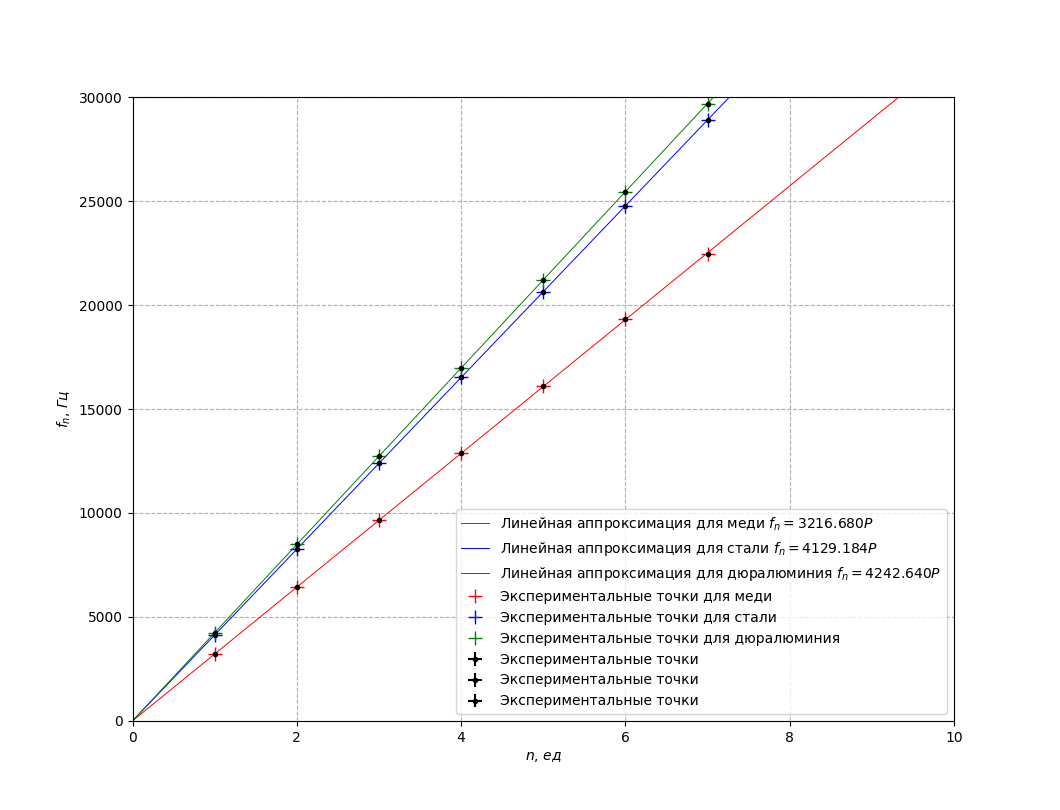
\includegraphics[width=1.1\textwidth]{graph.png}
	\caption{\textit{График зависимости $f_n$ от $n$}}
	\label{graph}
\end{figure}

\end{document}
